% ===================================================================
\chapter{Comparison with the Baseline}
\label{ch:vskiem}

Chapter~\ref{ch:kiem} set out what Kiem measured; Chapter~\ref{ch:results} set
out what this thesis measures. This chapter puts the two side by side. That is
less simple than it sounds, because every comparison has to cross two gaps at
once: different data and a different radar. Kiem's compression ratios come from
private recordings of a single-transmitter sensor with real-valued samples;
this thesis's come from a public twelve-transmitter cascade with complex
samples. Four questions cannot be answered across both gaps together:

\begin{enumerate}
\item Kiem reports a ratio of \num{3.25} for DRHE on his recordings; on
ColoRadar this thesis's DRHE reaches \num{3.75}. What actually sets the ratio,
and are the two numbers comparable? As a test of that question, this chapter
also runs this thesis's own chain on synthetic scenes of the kind Kiem
describes, and they compress to only about \num{1.1}
(Section~\ref{sec:kr_scaling}). A comparison has to explain all three
figures.
\item Kiem calls LPC ``the same approach as DRHE'' but less promising. The LPC of
this thesis is level with DRHE. Which is right?
\item Is the DRHE of this thesis the algorithm Kiem specified?
\item The hardware differs from his in every resource figure. Which differences
come from design decisions, and which from tools, devices and data?
\end{enumerate}

\noindent
The chapter answers them with two reconstructions. The first rebuilds Kiem's
MATLAB simulation \emph{from his text alone} --- his radar, his scene, his
processing chain, one transmitter --- and runs on it every coder discussed in
this thesis (Sections~\ref{sec:kr_built}--\ref{sec:kr_tdm}). It closes the
data gap for the first three questions. The second rebuilds his compression IP
in this thesis's tool flow; it is the subject of Chapter~\ref{ch:hwinterpret}
(Section~\ref{sec:hw_replica} onwards), which closes the tool and device gap
for the fourth question, and Section~\ref{sec:kc_replica} summarises what it
means for this comparison. With both in place, every result and claim of
his is compared with this thesis's in turn
(Sections~\ref{sec:kc_table}--\ref{sec:kc_summary}).

\section{Three kinds of comparison}
\label{sec:kc_kinds}

Not every pair of numbers can be compared directly, and the most common error
in comparing compression results is to compare numbers that measure different
things. Each comparison in this chapter is placed in one of three classes.

\begin{description}[leftmargin=!,labelwidth=30mm,style=nextline,font=\normalfont\bfseries]
\item[Like for like] The two numbers measure the same quantity of the same
thing, and a difference is a real difference. Examples: the arithmetic
specification of DRHE; post-route LUTs of two circuits built for the same
device.
\item[Through a bridge] The numbers come from different data or setups, but
something built for the purpose connects them: the rebuilt simulation of his
chain, or the rebuilt copy of his hardware.
\item[Not comparable] The numbers look alike but measure different things, and
no bridge closes the gap. Example: his CR on his recordings against this
thesis's on ColoRadar. For these the chapter explains what each number does
measure.
\end{description}

% -------------------------------------------------------------------
\section{Rebuilding Kiem's simulation}
\label{sec:kr_built}

The replication is a separate MATLAB code base that uses base MATLAB only and
shares no code with the evaluation chain of Chapter~\ref{ch:evaluation}. Its
stages follow Kiem's Figure~3.1 and are listed in Table~\ref{tab:kr_files} with
the section of his thesis each one implements.

\begin{table}[htbp]
\centering
\caption[Replication: stages and sources]{The rebuilt simulation, stage by
stage, with the part of Kiem's thesis each stage is built from.}
\label{tab:kr_files}
\small
\begin{tabular}{@{}p{42mm}p{62mm}p{28mm}@{}}
\toprule
File & Role & Kiem\\
\midrule
\texttt{kr\_config.m} & every parameter, with its source or ``ASSUMPTION'' & Tables 3.2, 3.3, 4.4; App.\ A\\
\texttt{kr\_generate\_adc.m} & beat signals of the targets, AWGN, 14-bit ADC; optional TDM interleaving & \S{}3.2.2\\
\texttt{kr\_calibrate\_noise.m} & ADC noise level that gives a chosen noise floor after NCI & Table 3.2\\
\texttt{kr\_preprocess\_fft.m} & shift to 32-bit full scale, Hanning, FFT$/N$, first half & \S{}3.2.1, \S{}4.3.3\\
\texttt{kr\_fp16.m}, \texttt{kr\_fx16.m} & FP16 reference; FX16 in two scalings & \S{}3.4.1\\
\texttt{kr\_second\_stage.m}, \texttt{kr\_detect.m} & Doppler FFT, NCI, noise threshold and local maxima & \S{}3.2.1\\
\texttt{kr\_metrics.m} & CR, FN\%, FP\%, NF, SNR against FP16 & \S{}3.4.2\\
\texttt{kr\_drhe\_*.m} & DRHE model prediction and its inverse & \S{}3.5.3, \S{}3.5.4\\
\texttt{kr\_bits\_s4.m}, \texttt{kr\_bits\_r4s4.m} & $S_4$ coder (fixed or ideal dictionary); R4S4 + run-length coder & Table 3.7, \S{}2.7.3, \S{}3.5.1\\
\texttt{kr\_lpc\_raw.m} & LPC-Huffman of \cite{meucci2022}: fast-time prediction of raw ADC & \S{}2.7.4\\
\texttt{kr\_lpc\_fft.m} & this thesis's slow-time LPC, for comparison & ---\\
\texttt{kr\_lossy.m} & approximations of CMPRA/B and EGE10/8/6/4 & \S{}2.7.1, \S{}2.7.2\\
\texttt{run\_kiem\_replication.m} & the whole workflow at two noise levels & Fig.\ 3.1\\
\bottomrule
\end{tabular}
\end{table}

Every lossless path is decoded and compared with its input on every run; none
is assumed lossless. One detail of the DRHE decoder is specific to a
floating-point model. MATLAB's \texttt{round} returns $-0$ for small negative
values, and $\mathrm{atan2}(-0, x<0) = -\pi$ while
$\mathrm{atan2}(+0, x<0) = +\pi$. An encoder that saw $-0$ and a decoder that
rebuilds the value as an integer, and so sees $+0$, would form phase
predictions $2\pi$ apart. The FX16 quantiser of the replication therefore
normalises $-0$ to $+0$. A hardware implementation never meets this, because
integers have no negative zero, but a floating-point model of one can.

\subsection{The radar and the scene}
\label{sec:kr_scene}

The radar is Kiem's Table~3.2: one MMIC, \textbf{one transmitter}, four
receivers, 1024 samples per ramp, 512 ramps, a 14-bit ADC. The scene has his
five targets at range bins [100, 150, 150, 200, 400] and Doppler bins [50, 50,
100, 200, 250] with amplitudes [0.8, 0.3, 0.4, 0.5, 0.7] of full scale, and
white Gaussian noise set so that the noise floor after NCI is his
$-75$\,dBFS. Figure~\ref{fig:kr_scene} shows it; it is visibly the scene of his
Figures~3.5 and~3.7.

\begin{figure}[htbp]
\centering
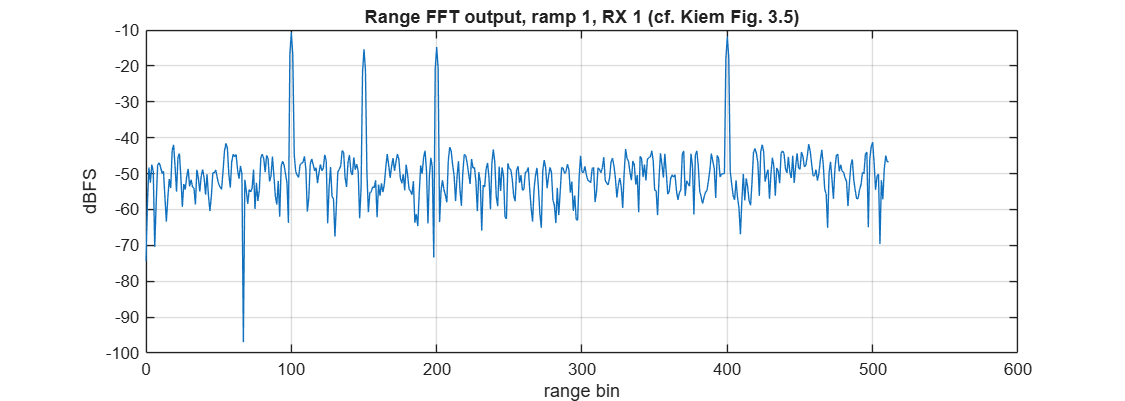
\includegraphics[width=0.49\textwidth]{fig_kr_rangefft.png}\hfill
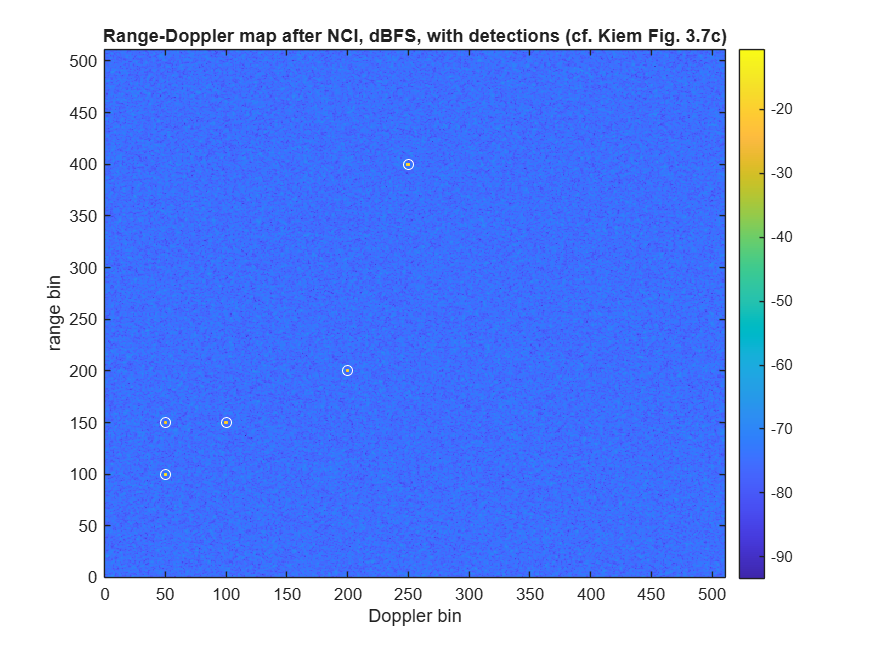
\includegraphics[width=0.46\textwidth]{fig_kr_rdmap.png}
\caption[The rebuilt scene]{Kiem's Table~3.2 scene as rebuilt. Left: range
FFT of ramp 1, receiver 1 (compare his Figure~3.5). Right: range--Doppler map
after NCI with the five reference detections circled (compare his
Figure~3.7c).}
\label{fig:kr_scene}
\end{figure}

\subsection{Where Kiem's text leaves a choice}
\label{sec:kr_assump}

Seven parameters are not given in his thesis. Each is set in one place
(\texttt{kr\_config.m}), marked there as an assumption, and can be changed.

\begin{description}[leftmargin=!,labelwidth=30mm,style=nextline,font=\normalfont\bfseries]
\item[Target angles] Not given. Fixed, distinct angles
($-30^\circ$, $-10^\circ$, $0^\circ$, $15^\circ$, $40^\circ$) on a
half-wavelength array, so the four receive channels differ.
\item[Amplitudes] His five amplitudes sum to 2.7 of full scale, which a 14-bit
ADC cannot hold without clipping. They are scaled together so the worst-case
sum just fits.
\item[FX16 scaling] Two modes, both fixed and independent of the data. In
\emph{hw}, the default, the FX16 code is the top 16 bits of the 32-bit FFT
word, which is what his FFT core delivers: the full scale of the \emph{word}
maps to \num{32767}. In \emph{full scale}, the scaling of this thesis's chain
(Equation~\eqref{eq:scale}), the spectral peak of a full-scale \emph{sinusoid}
maps to \num{32767}. They differ by exactly a factor of four, because a
full-scale real sinusoid reaches only a quarter of the word's full scale after
the range FFT: the Hanning window's coherent gain halves it, and a real
sinusoid's amplitude is split equally between its positive- and
negative-frequency bins, which halves it again. Equation~\eqref{eq:scale}
divides both factors out.
\item[0\,dBFS] Not defined in his thesis. The NCI power of a full-scale
sinusoid through the whole chain is the default; the power of a unit value in
the 32-bit word is also reported, and reads \SI{12.0}{\decibel} lower.
\item[Detector] Noise estimate the mean dB of the lowest \SI{75}{\percent} of
cells; threshold \SI{15}{\decibel} above it; 8-neighbour local maxima --- the
detector of Section~\ref{sec:refchain}.
\item[Noise floor and SNR] The noise floor is the mean dB outside a
$5\times5$ patch around each detection; SNR is the RMS peak power in dB minus it,
as in his Section~3.4.2.
\item[LPC-Huffman of Meucci and Mancuso] Order not given, so $p = 1 \ldots 10$
is swept; one coefficient set per chirp and receiver, sent as 32-bit floats;
the Huffman dictionary counted at 21 bits per symbol used.
\end{description}

\noindent
His lossy schemes cannot be reproduced exactly, because their bit layouts are
proprietary. They are approximated --- CMPRA and CMPRB as block floating point
with one 4-bit exponent per 256-bit word, EGE-$k$ as blocks of eight complex
bins with an 8-bit header and least significant bits dropped to meet CR
$16/k$ --- and are included for completeness rather than as evidence.

% -------------------------------------------------------------------
\section{Results at Kiem's noise level}
\label{sec:kr_m75}

Table~\ref{tab:kr_m75} runs the complete workflow at the $-75$\,dBFS of his
Table~3.2 and sets his published Table~3.5 beside it. The published numbers are
from his real recordings, not from this scene; they are there to be read
against, not matched.

\begin{table}[htbp]
\centering
\caption[Replication at $-75$\,dBFS]{Kiem's workflow on his Table~3.2 scene at
his $-75$\,dBFS noise floor, beside his Table~3.5. ADC noise
$\sigma = 375.9$ codes; FX16 noise \num{20.35}\,LSB; five reference detections.
``(approx.)'' marks schemes approximated because their exact layout is
proprietary.}
\label{tab:kr_m75}
\footnotesize
\setlength{\tabcolsep}{3.5pt}
\begin{tabular}{@{}lrrrrr@{\hskip 12pt}rrr@{}}
\toprule
& \multicolumn{5}{c}{\textbf{replication}} & \multicolumn{3}{c}{\textbf{Kiem, real data}}\\
\cmidrule(lr){2-6}\cmidrule(lr){7-9}
Algorithm & CR & FN\% & FP\% & NF & SNR & CR & FN\% & FP\%\\
\midrule
FP16 (reference)                   & 1.00 & 0 & 0 & $-75.00$ & 61.50 & 1.00 & 0 & 0\\
FX16                               & 1.00 & 0 & 0 & $-75.00$ & 61.50 & 1.00 & 0.59 & 1.18\\
CMPRA (approx.)                    & 2.00 & 0 & 0 & $-74.86$ & 61.36 & 2.00 & 0.59 & 0.59\\
CMPRB (approx.)                    & 4.00 & 0 & 13980 & $-75.56$ & 40.55 & 4.00 & 7.69 & 4.73\\
EGE10 (approx.)                    & 1.60 & 0 & 0 & $-75.00$ & 61.50 & 1.60 & 1.18 & 1.18\\
EGE8 (approx.)                     & 2.00 & 0 & 0 & $-74.98$ & 61.48 & 2.00 & 2.37 & 2.37\\
EGE6 (approx.)                     & 2.67 & 0 & 0 & $-74.79$ & 61.29 & 2.67 & 7.69 & 7.10\\
EGE4 (approx.)                     & 4.00 & 0 & 680 & $-74.71$ & 52.31 & 4.00 & 40.24 & 26.63\\
\textbf{DRHE, R4S4 + RLE}          & \textbf{2.28} & 0 & 0 & $-75.00$ & 61.50 & \textbf{3.25} & 0.59 & 1.18\\
DRHE, $S_4$ only, ideal dictionary & 2.28 & 0 & 0 & $-75.00$ & 61.50 & 3.24 & 0.59 & 1.18\\
DRHE, $S_4$, Kiem's fixed dictionary & 1.85 & 0 & 0 & $-75.00$ & 61.50 & (3.17 HW) & & \\
LPC-Huffman, raw ADC \cite{meucci2022}, $p=10$  & 1.32 & 0 & 0 & $-75.00$ & 61.50 & (2.056 in \cite{meucci2022}) & & \\
LPC, slow time (this thesis)       & 2.06 & 0 & 0 & $-75.00$ & 61.50 & & & \\
No prediction, fixed dictionary    & 2.03 & 0 & 0 & $-75.00$ & 61.50 & & & \\
\bottomrule
\end{tabular}
\end{table}

\noindent
Three things stand out.

\paragraph{DRHE compresses to 2.28 on Kiem's own scene, not 3.25.} The scene
is his, the chain is his and the algorithm is his (Section~\ref{sec:kc_audit}
shows it is exactly his). The ratio is not, which already shows that his 3.25
is a property of his recordings rather than of his illustrative scene.

\paragraph{The detection columns do not resemble his.} This scene has five
targets 60 to \SI{74}{\decibel} above the noise; his recordings had about 170
detections at \SI{22}{\decibel}. With five detections, one miss would be
\SI{20}{\percent}, so FN and FP are not comparable at all. The same high SNR is
why the approximated lossy schemes produce large false-discovery rates here: at
\SI{60}{\decibel} SNR a 3-bit mantissa leaves quantisation spurs in the
range--Doppler map that are 20 to \SI{40}{\decibel} above the noise and are
detected as targets. Those FP percentages describe this scene, not the schemes.

\paragraph{Prediction is doing almost nothing.} No prediction at all gives 2.03
through the fixed dictionary; DRHE gives 1.85 and the slow-time LPC 2.06. In a
scene that is \SI{99.99}{\percent} noise cells there is nothing to predict:
noise at ramp $m-1$ says nothing about noise at ramp $m$.
Section~\ref{sec:kr_sweep} shows that this holds at every noise level.

% -------------------------------------------------------------------
\section{The noise level at which DRHE gives 3.25}
\label{sec:kr_m88}

On a white-noise scene the compression ratio depends on one thing above all:
the standard deviation of the noise in FX16 least significant bits. A bisection
on the noise floor (\texttt{kr\_find\_nf\_for\_cr.m}) finds the level at which
DRHE with run-length coding gives Kiem's 3.25: $-87.9$\,dBFS, where the ADC
noise is 85.4 codes and the FX16 noise \num{4.63}\,LSB.
Table~\ref{tab:kr_m88} gives the full workflow there.

\begin{table}[htbp]
\centering
\caption[Replication at $-87.9$\,dBFS]{The same workflow at the noise floor
where DRHE reproduces Kiem's 3.25. ADC noise $\sigma = 85.4$ codes; FX16 noise
\num{4.63}\,LSB. Detection metrics are omitted: every lossless row equals
FX16's (no misses, no false detections).}
\label{tab:kr_m88}
\small
\begin{tabular}{@{}lrr@{}}
\toprule
Coder & replication & Kiem\\
\midrule
DRHE, R4S4 + RLE, ideal Huffman     & \textbf{3.25} & \textbf{3.25} (his Table 3.5)\\
DRHE, $S_4$ only, ideal Huffman     & \textbf{3.24} & \textbf{3.24} (his Table 3.6)\\
DRHE, $S_4$, Kiem's fixed dictionary & 3.23 & 3.17 (hardware, different FFT)\\
LPC-Huffman on raw ADC \cite{meucci2022}, $p=10$ & 1.54 & not run (2.056 in \cite{meucci2022})\\
LPC, slow time, fixed dictionary    & 3.38 & ---\\
LPC, slow time, ideal Huffman       & 3.43 & ---\\
No prediction, fixed dictionary     & 3.26 & ---\\
No prediction, R4S4 + RLE           & 3.38 & ---\\
\bottomrule
\end{tabular}
\end{table}

\noindent
At this one noise level the replication reproduces Kiem's DRHE pattern
exactly: 3.25 with run-length coding, 3.24 without (his Table~3.6), and almost
no loss from fixing the dictionary (3.23). It reproduces his observation that
run-length coding adds nearly nothing. But the operating point was
\emph{chosen} to give 3.25; it is not a prediction. And it sits
\SI{17.2}{\decibel} below the $-70.7$\,dBFS noise floor he reports with that
3.25, a discrepancy that Section~\ref{sec:kr_nfcr} examines.

% -------------------------------------------------------------------
\section{Compression ratio across noise levels}
\label{sec:kr_sweep}

Figure~\ref{fig:kr_sweep} sweeps the noise floor of the same scene from
$-120$ to $-60$\,dBFS, for both FX16 scalings
(\texttt{kr\_noise\_sweep.m}). Kiem's published result is placed on it, and so
are the results of the synthetic-scene test of Section~\ref{sec:kr_scaling},
which runs this thesis's own chain.

\begin{figure}[htbp]
\centering
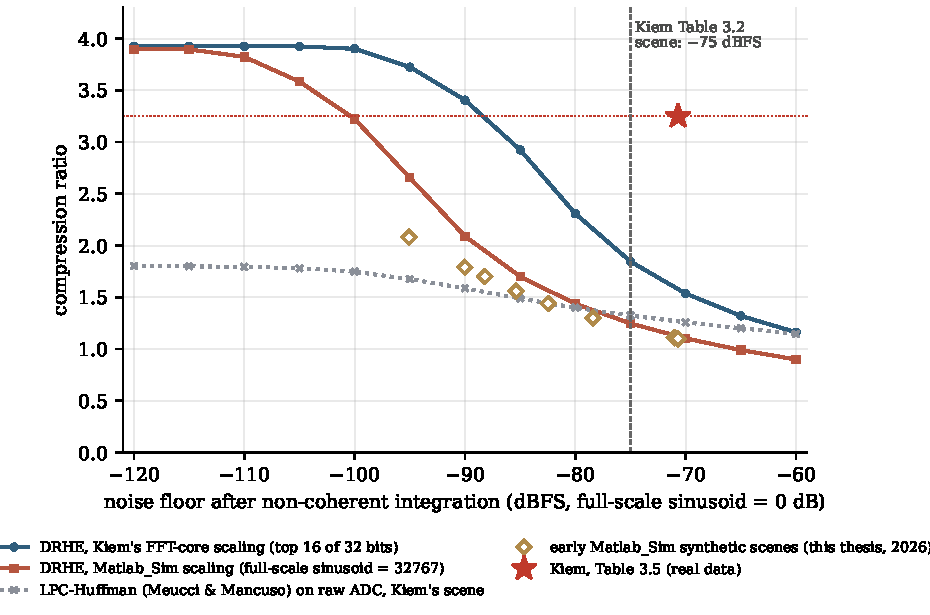
\includegraphics[width=\textwidth]{fig_kr_sweep.pdf}
\caption[CR against noise floor on Kiem's scene]{Compression ratio against
noise floor on Kiem's Table~3.2 scene with one transmitter. Blue: DRHE with
Kiem's fixed dictionary and his FFT core's scaling. Red: the same with the
full-scale scaling of this thesis's chain, four times larger. Grey: LPC-Huffman
of \cite{meucci2022} on raw ADC. Diamonds: the synthetic-scene test of
Section~\ref{sec:kr_scaling}, run through this thesis's chain. Star: Kiem's published 3.25 at $-70.7$\,dBFS, which lies
\SI{17}{\decibel} to the right of where his own scaling's curve passes 3.25.}
\label{fig:kr_sweep}
\end{figure}

The curves have three regimes.

\begin{itemize}
\item \textbf{Very low noise} (left). The FX16 noise rounds to zero, the
residuals are nearly all zero, and the fixed dictionary's floor takes over:
every value costs at least four bits (Section~\ref{sec:huffman}), so the ratio
saturates just below 4.0 (3.92). With run-length coding and an ideal dictionary
it would grow without limit (82 at $-140$\,dBFS), because long runs of zeros
cost almost nothing; that regime is irrelevant to a real radar.
\item \textbf{The transition} (centre). Each \SI{6}{\decibel} of extra noise
doubles the noise in LSB, adds about one bit to every residual and lowers the
ratio.
\item \textbf{High noise} (right). Every value carries several bits of noise
and the ratio falls towards 1.
\end{itemize}

\noindent
The two scalings produce the same curve shifted by \SI{12}{\decibel}, as a
factor of four in amplitude must. Along both curves, no prediction and the
slow-time LPC stay within about ten per cent of DRHE either way, and with the
fixed dictionary no prediction is often the better of the two
(Tables~\ref{tab:kr_m75} and~\ref{tab:kr_m88}): on white noise the predictor is
not what sets the ratio. The diamonds, from this thesis's chain, fall on the
red curve; the next section explains why.

% -------------------------------------------------------------------
\section{This thesis's chain on synthetic scenes}
\label{sec:kr_scaling}

The replication makes possible a direct test of how much of a compression ratio
belongs to the chain rather than to the algorithm. Synthetic scenes of the kind
Kiem's thesis describes --- a handful of point targets in white Gaussian noise
--- were generated at eight noise floors between $-95$ and $-70.7$\,dBFS and put
through this thesis's own MATLAB chain (Section~\ref{sec:refchain}), with its
full-scale FX16 scaling, DRHE and Kiem's fixed dictionary. They are the
diamonds of Figure~\ref{fig:kr_sweep}. Near the $-70.7$\,dBFS that Kiem
reports, they compress to only \num{1.10}--\num{1.12}; at $-95$\,dBFS they
reach \num{2.08}. Running this thesis's chain on scenes of Kiem's kind therefore
gives about \num{1.1}, a third of his \num{3.25}, with the same algorithm and
the same dictionary. The replication explains why. Table~\ref{tab:kr_scaletab}
runs Kiem's scene at three noise floors with both scalings.

\begin{table}[htbp]
\centering
\caption[FX16 scaling and noise floor]{DRHE and the other coders on Kiem's
scene for both FX16 scalings. ``Noise'' is the standard deviation of FX16 codes
in noise-only range bins. ``DRHE, fixed'' uses Kiem's fixed dictionary;
``R4S4'' is the run-length coder with an ideal dictionary.}
\label{tab:kr_scaletab}
\small
\setlength{\tabcolsep}{5pt}
\begin{tabular}{@{}lrrrrrr@{}}
\toprule
FX16 scaling & NF (dBFS) & noise (LSB) & DRHE, fixed & DRHE, R4S4 & LPC & no pred.\\
\midrule
hw (Kiem's FFT core) & $-70.7$ & 33.4 & 1.57 & 2.07 & 1.73 & 1.71\\
hw                   & $-75.0$ & 20.4 & 1.85 & 2.28 & 2.06 & 2.03\\
hw                   & $-87.9$ & 4.6  & \textbf{3.24} & 3.25 & 3.38 & 3.26\\
full scale (this thesis) & $-70.7$ & 133.4 & \textbf{1.12} & 1.64 & 1.20 & 1.19\\
full scale           & $-75.0$ & 81.3 & 1.25 & 1.78 & 1.34 & 1.32\\
full scale           & $-87.9$ & 18.4 & 1.91 & 2.32 & 2.13 & 2.08\\
\bottomrule
\end{tabular}
\end{table}

\noindent
The row ``full scale, $-70.7$\,dBFS'' gives \num{1.12}, the same ratio as
this thesis's chain on its synthetic scenes (\num{1.10}--\num{1.12}),
reproduced in an independent code base from nothing but Kiem's text and the
full-scale scaling. Two factors
multiply to produce it:

\begin{itemize}
\item \textbf{The scaling, a factor of four.} Both chains use a fixed
full-scale scaling, but they calibrate it to different references. This
thesis's maps the peak of a full-scale sinusoid to \num{32767}; Kiem's core
keeps the top 16 bits of the 32-bit FFT word, in which the same sinusoid peaks
at about \num{8191}, a quarter of the word's full scale
(Section~\ref{sec:kr_assump}). The same noise therefore occupies four times as
many LSB here, about two more bits per value.
\item \textbf{The noise floor, a factor of seven.} Matching Kiem's stated
$-70.7$\,dBFS with white noise gives 33\,LSB even with his scaling; his CR of
3.25 needs about 4.6\,LSB.
\end{itemize}

\noindent
Together: 133\,LSB of noise where his result implies about 5, some thirty times
more. It is tempting to explain the low ratio by saying that white noise lacks
the slow-time correlation DRHE needs. White noise is indeed unpredictable, but
that is not what sets the ratio: the no-prediction column shows the same ratios
without any predictor. The ratio is set by how many bits of noise each value
carries, and that is fixed by the scaling and the noise level before any coder
runs. The same mechanism, seen from the other side, is why the ColoRadar capture
compresses as well as it does: its FX16 codes occupy fewer than ten of the
sixteen bits (Section~\ref{sec:decomp}).

% -------------------------------------------------------------------
\section{Kiem's noise floor and his compression ratio do not agree}
\label{sec:kr_nfcr}

The replication cannot make Kiem's reported noise floor and his reported
compression ratio hold together on a white-noise scene, under any reading of
his text. With his FFT scaling, CR 3.25 needs $-87.9$\,dBFS by the
full-scale-sinusoid reference or $-99.9$\,dBFS by the unit reference; he
reports $-70.7$\,dBFS. These are the only two references his text suggests, and
the second only widens the gap.

\subsection{His dictionary says what his residuals looked like}
\label{sec:kr_fingerprint}

Kiem built his fixed Huffman dictionary from the $S_4$ statistics of his own
residuals (Section~\ref{sec:kc_adapt}). A Huffman code is optimal only for
the distribution it was built from, so its lengths can be read backwards.
Table~\ref{tab:kr_fp} (\texttt{kr\_dictionary\_fingerprint.m}) codes
integer-rounded Gaussian residuals of increasing spread with his dictionary and
with the ideal code for each spread.

\begin{table}[htbp]
\centering
\caption[What Kiem's dictionary was built for]{Kiem's fixed dictionary
against an ideal Huffman code on Gaussian residuals. The overhead is smallest
where the dictionary matches the data it was made from.}
\label{tab:kr_fp}
\small
\begin{tabular}{@{}rrrrr@{}}
\toprule
Residual std (LSB) & CR, Kiem's dictionary & CR, ideal code & overhead & commonest $S_4$\\
\midrule
1   & 4.00 & 6.80 & \SI{70.1}{\percent} & 1\\
2   & 3.92 & 4.84 & \SI{23.2}{\percent} & 2\\
4   & 3.60 & 3.75 & \SI{4.1}{\percent}  & 2\\
5   & 3.46 & 3.48 & \SI{0.6}{\percent}  & 3\\
\textbf{6}   & \textbf{3.33} & \textbf{3.33} & \textbf{\SI{0.0}{\percent}}  & 3\\
\textbf{7}   & \textbf{3.20} & \textbf{3.20} & \textbf{\SI{0.0}{\percent}}  & 3\\
\textbf{8}   & \textbf{3.07} & \textbf{3.07} & \textbf{\SI{0.1}{\percent}}  & 3\\
10  & 2.82 & 2.88 & \SI{2.2}{\percent}  & 4\\
15  & 2.38 & 2.63 & \SI{10.2}{\percent} & 4\\
20  & 2.12 & 2.45 & \SI{15.8}{\percent} & 5\\
33  & 1.76 & 2.21 & \SI{25.6}{\percent} & 5\\
\bottomrule
\end{tabular}
\end{table}

\noindent
The dictionary is optimal for residuals with a standard deviation of 6 to
8\,LSB and costs \SI{26}{\percent} for the 33\,LSB that his reported noise floor
would give on white noise. Its fingerprint agrees with his CR of 3.25 and with
his residual histograms (his Figures~3.9--3.10, ``most values'' within
$\pm 40$); it does not agree with a white-noise floor at $-70.7$\,dBFS. The same
table explains, from the other end, why the dictionary is a poor fit for the
lag-$\nTx$ residuals of ColoRadar: more than four fifths of those fall in
categories 0 to 2 (Table~\ref{tab:dictshare}), the region of the first two rows, where the
fixed dictionary's overhead is largest.

\subsection{The most likely reconciliation}

His Table~3.5 was measured on real recordings. In real data the ``mean of the
noisy part of the signal in dB'' can be raised by clutter, leakage, sidelobes
and slowly varying returns in the cells the estimator averages, while most cells
--- which set the compression ratio --- sit much lower. In a white-noise
simulation the noise floor and the per-cell noise are the same number, so
matching his noise floor forces far too much noise into every cell. This
reconciliation fits every figure available: his ratio, his dictionary and his
histograms. It cannot be confirmed without his data or code, and it is reported
as an inference, not a finding.

% -------------------------------------------------------------------
\section{LPC-Huffman, the method Kiem excluded}
\label{sec:kr_lpcraw}

\texttt{kr\_lpc\_raw.m} implements LPC-Huffman as Kiem describes it: a $p$-th
order predictor of each raw ADC sample from the previous $p$ samples of the same
chirp, Levinson--Durbin coefficients per chirp and receiver, sent as 32-bit
floats, and a Huffman code built from the residuals. The decoder runs sample by
sample and the round trip is checked.

\begin{table}[htbp]
\centering
\caption[LPC-Huffman of Meucci and Mancuso by order]{LPC-Huffman on the raw ADC
samples of Kiem's scene, by predictor order (CR including the dictionary). Five
real sinusoids need up to ten poles.}
\label{tab:kr_lpcorder}
\small
\begin{tabular}{@{}rrrrr@{}}
\toprule
& \multicolumn{2}{c}{$-75$\,dBFS} & \multicolumn{2}{c}{$-87.9$\,dBFS}\\
\cmidrule(lr){2-3}\cmidrule(lr){4-5}
$p$ & CR & residual std (codes) & CR & residual std (codes)\\
\midrule
1  & 1.174 & 2686 & 1.176 & 2660\\
2  & 1.172 & 2682 & 1.174 & 2655\\
4  & 1.204 & 2014 & 1.208 & 1966\\
6  & 1.312 & 921  & 1.388 & 602\\
8  & 1.310 & 899  & 1.426 & 506\\
10 & \textbf{1.324} & 799 & \textbf{1.543} & 318\\
\bottomrule
\end{tabular}
\end{table}

\noindent
On Kiem's own scene, at either noise level, the method he excluded loses to
DRHE by a wide margin (1.32 against 1.85--2.28; 1.54 against 3.23--3.25), and
it stays below 1.8 across the whole sweep (Figure~\ref{fig:kr_sweep}).
\textbf{For the LPC he meant, Kiem's ranking holds.} It holds for a reason that
has little to do with the predictor.

\paragraph{Raw-ADC coding must keep bits the FX16 step has already discarded.}
Kiem's chain shifts the 14-bit samples left by 18 bits, windows them, takes the
FFT divided by $N$ and keeps the top 16 bits. White ADC noise of standard
deviation $\sigma$ codes therefore reaches the FX16 word with standard
deviation
\begin{equation}
\label{eq:kr_noisemap}
\sigma_{\mathrm{FX16}} = \sigma \cdot \frac{2^{18}}{2^{16}} \cdot
\frac{\sqrt{\sum_k w_k^2 / 2}}{N}
= \sigma \cdot 4 \cdot \sqrt{\frac{0.375}{2 \times 1024}} = 0.0541\,\sigma,
\end{equation}
using $\sum_k w_k^2 \approx 0.375N$ for a Hanning window. The simulation
measures exactly this ratio: 375.9 codes become 20.35\,LSB and 85.4 codes become
4.63\,LSB. The FFT scaling and the truncation to 16 bits thus discard
$\log_2(1/0.0541) \approx 4.2$ bits of noise per value before DRHE ever sees the
data. A lossless coder of the raw samples must keep them. At $-87.9$\,dBFS even a
perfect predictor would leave a residual of at least the ADC noise, 85 codes,
whose entropy is about $\log_2(85\sqrt{2\pi e}) \approx 8.5$ bits, capping the
ratio near $16/8.5 \approx 1.9$; the prediction filter then amplifies white
noise, and the measured ratio is 1.54.

So the comparison Kiem made on paper is between a lossless coder of the ADC
stream and a lossless coder of already-truncated data. The truncation is the
lossy step, and his Table~3.5 shows its cost in the FX16 row
(\SI{0.59}{\percent} missed, \SI{1.18}{\percent} spurious). DRHE inherits that
cost; LPC-Huffman on raw ADC does not.

\paragraph{The coefficient method is not the problem.} The Levinson--Durbin
(autocorrelation) method is biased for pure sinusoids over a finite record; the
covariance (true least-squares) method is not. Replacing one with the other
(\texttt{kr\_lpc\_raw\_method\_check.m}) raises the ratio only when there is
almost no noise --- from 1.83 to 6.51 at $-140$\,dBFS, $p = 10$ --- and changes
nothing at the noise levels that matter: 1.56 against 1.59 at $-87.9$\,dBFS and
1.34 against 1.34 at $-75$\,dBFS.

\paragraph{The slow-time LPC is a different matter.} On the same scene the LPC
of this thesis --- same domain and coder as DRHE --- gives 2.06 against DRHE's
1.85 at $-75$\,dBFS and 3.38 against 3.23 at $-87.9$\,dBFS, and it stays level
with or slightly above DRHE across the sweep from $-95$\,dBFS upwards. On
Kiem's scene, the controlled comparison comes out the other way from his
remark.

% -------------------------------------------------------------------
\section{Adding transmitters}
\label{sec:kr_tdm}

The replication can also do what Kiem's radar cannot: interleave the ramps
over twelve transmitters, each at its own position in a virtual array, as in
the ColoRadar cascade (\texttt{kr\_tdm\_experiment.m}). Two scenes are used:
Kiem's five-target scene, and a denser one that is \emph{not} from Kiem --- 300
slowly moving scatterers between $-70$ and \SI{-30}{\decibel} of full scale at
random angles, a stand-in for a real indoor scene.

\begin{table}[htbp]
\centering
\caption[One against twelve transmitters]{DRHE (fixed dictionary) and the other
coders with one transmitter and with twelve interleaved, predicting from the
previous ramp (lag 1) or from the previous ramp of the same transmitter
(lag 12).}
\label{tab:kr_tdm}
\small
\begin{tabular}{@{}llrrrr@{}}
\toprule
Scene, noise floor & radar, lag & DRHE & DRHE+RLE & LPC & no pred.\\
\midrule
Kiem, $-75$\,dBFS  & 1 TX, lag 1   & 1.850 & 2.285 & 2.070 & 2.036\\
                   & 12 TX, lag 1  & 1.836 & 2.262 & 2.051 & 2.036\\
                   & 12 TX, lag 12 & 1.859 & 2.283 & 2.056 & 2.036\\
\midrule
Kiem, $-95$\,dBFS  & 1 TX, lag 1   & 3.726 & 4.237 & 3.760 & 3.603\\
                   & 12 TX, lag 1  & 3.641 & 4.120 & 3.666 & 3.603\\
                   & 12 TX, lag 12 & 3.694 & 4.208 & 3.665 & 3.603\\
\midrule
Dense, $-75$\,dBFS & 1 TX, lag 1   & 1.772 & 2.203 & 1.960 & 1.656\\
                   & 12 TX, lag 1  & 1.647 & 2.066 & 1.798 & 1.657\\
                   & 12 TX, lag 12 & 1.689 & 2.110 & 1.840 & 1.657\\
\midrule
Dense, $-95$\,dBFS & 1 TX, lag 1   & \textbf{3.398} & 3.516 & 3.596 & 1.952\\
                   & 12 TX, lag 1  & \textbf{2.371} & 2.514 & 2.462 & 1.955\\
                   & 12 TX, lag 12 & \textbf{2.560} & 2.673 & 2.712 & 1.955\\
\bottomrule
\end{tabular}
\end{table}

\noindent
On Kiem's scene the transmitters make almost no difference, because there is
almost nothing but noise to predict. On the dense scene at low noise, prediction
earns its keep --- DRHE 3.40 against 1.95 without prediction --- and TDM
interleaving costs it a third of its ratio (2.37). Predicting from the same
transmitter recovers part of the loss (2.56). The recovery is only partial in
this synthetic scene, for two likely reasons: each transmitter's predictor
starts from zero, so there are twelve cold starts per frame instead of one; and
the synthetic scatterers move, so each lag-12 prediction spans a Doppler step
twelve times larger than a lag-1 prediction on a single-transmitter radar. On
ColoRadar, whose scene changes slowly, the same change of lag turns a
\SI{4.9}{\percent} loss against no prediction into a \SI{7.8}{\percent} gain
(Section~\ref{sec:predaxisres}). The mechanism is the same in both: on a
TDM-MIMO radar, a slow-time predictor carried over from a single-transmitter
design must be told which earlier ramp belongs to the same antenna.

% -------------------------------------------------------------------
\section{The DRHE algorithm, line by line}
\label{sec:kc_audit}

Kiem's Section~3.5.3 specifies the final scheme and his Section~4.3.4 the
hardware form of it. Table~\ref{tab:kc_audit} takes every element in turn and
compares it with this thesis's MATLAB model and its HLS design.

\begin{table}[p]
\centering
\caption[DRHE audit against Kiem's specification]{Every element of Kiem's final
DRHE scheme (his \S{}3.5.3, \S{}3.5.4 and \S{}4.3.4) against this thesis's MATLAB
model and HLS design. The letters in the last column refer to the explanations
in Section~\ref{sec:kc_why}.}
\label{tab:kc_audit}
\scriptsize
\renewcommand{\arraystretch}{1.25}
\setlength{\tabcolsep}{3pt}
\begin{tabular}{@{}>{\raggedright}p{0.15\textwidth}>{\raggedright}p{0.26\textwidth}>{\raggedright}p{0.17\textwidth}>{\raggedright}p{0.24\textwidth}>{\raggedright\arraybackslash}p{0.10\textwidth}@{}}
\toprule
Element & Kiem & MATLAB model & HLS design & Same?\\
\midrule
Input & FX16 range FFT, first $N/2$ bins, per RX, ramp by ramp & same & same (128-bit AXIS, 4 RX) & yes\\
Cartesian to polar & $a = \sqrt{re^2+im^2}$, $\theta = \mathrm{atan2}(im, re)$ & same, double & same, single precision & yes; (b)\\
Magnitude, his Eq.~3.5 & $\hat a[m] = \alpha\hat a[m-1] + (1-\alpha)a[m-1]$ & same, at lag $L$ & same, at lag $L$ & yes; (e)\\
Phase, his Eq.~3.6 & $\hat\theta[m] = \beta\hat\theta[m-1] + (2-\beta)\theta[m-1] - \theta[m-2]$ & same, at lag $L$ & same, at lag $L$ & yes; (e)\\
Phase wrap & once into $[-\pi,\pi]$ (his listing, \S{}4.3.4) & same & same & yes\\
$\alpha$, $\beta$ & 0.6, 0.4 (his Table 4.4) & same & same & yes\\
Polar to Cartesian & rounded to integer (\texttt{AP\_RND}) & \texttt{round} & \texttt{roundf} & yes\\
Difference, his Eq.~3.7 & $X - \hat X$ in 16-bit two's complement & \texttt{wrap\_int16} & \texttt{wrap\_int16} & yes\\
Initial state & zero (\S{}3.5.4) & zero per frame & zero; each transmitter's state reset on its first ramp of every frame & yes; (c)\\
State update & from the input sample & from the input & from the reconstructed sample & \textbf{changed}; (a)\\
Run-length code & removed (\S{}3.5.1) & none & none & yes\\
Size category $S_4$ & his Table 3.7, 0--15 & $\lfloor\log_2|v|\rfloor+1$, capped at 15 & same regions, by comparison & yes\\
APPEND & $v$ if $v>0$; $v + 2^{S_4} - 1$ if $v<0$ & counted & same formula & yes\\
Residual $-32768$ & no code ($S_4 = 15$ spans $\pm[16384, 32767]$); not addressed & counted as $S_4 = 15$ & saturated to $-32767$ & \textbf{changed}; (a)\\
Dictionary & fixed, his Appendix A & same 16 lengths & same codes, bit-reversed & yes; (d)\\
Arithmetic & fixed point: \texttt{ap\_ufixed<16,16>}, \texttt{ap\_fixed<16,3>}, \texttt{ap\_fixed<32,4>} & double & single-precision float & \textbf{changed}; (b)\\
Output packing & 58-bit word per channel into 256-bit AXIS & bit count only & 512-bit accumulator, 256-bit AXIS & layout; (d)\\
Prediction lag & ramp $m-1$ (one TX) & $L = \nTx$; $L = 1$ for one TX & $L = \nTx$ (lag-1 variant: $L = 1$) & extension; (e)\\
\bottomrule
\end{tabular}
\end{table}

\subsection{Verification that the algorithm is the same}
\label{sec:kr_crosscheck}

Agreement on paper is checked by agreement in output, at every link from Kiem's
text to the board.

\begingroup\sloppy
\begin{itemize}
\item \textbf{Kiem's text to this thesis's MATLAB model.} The
replication's DRHE, \texttt{kr\_drhe\_encode.m}, written from Kiem's Section~3.5.3 without
reference to this thesis's code, and this thesis's MATLAB DRHE model at lag 1,
as a single-transmitter scene requires, were run on the same FX16 frames of the
replicated scene. The comparison script,
\texttt{kr\_crosscheck\_matlabsim.m}, is the one file of the replication that
touches the main code base, and only to read it. They produce
\emph{identical} residuals and identical bit counts: \num{18186374} bits at
$-75$\,dBFS and \num{10370342} at $-87.9$\,dBFS, a difference of zero in
each.
\item \textbf{MATLAB model to HLS.} The HLS designs reproduce the MATLAB
models' bit counts on all 50 ColoRadar frames, apart from the zero padding of
the last 256-bit output word (Section~\ref{sec:verifres}); this holds for the
lag-$\nTx$ design and for its lag-1 variant, whose datapath is identical apart
from the indexing of the state.
\item \textbf{HLS to an independent implementation.} A third implementation, in
Python, written from the specification without reusing any code, reproduces the
HLS bit count of every frame exactly (Section~\ref{sec:indep}).
\item \textbf{HLS to the board.} The FPGA's compressed output is byte-identical
to the C-simulation on all 50 frames (Section~\ref{sec:verifres}).
\end{itemize}
\endgroup

\noindent
The chain from Kiem's specification to the hardware is therefore closed at
every link. The DRHE of this thesis is Kiem's DRHE, extended in one documented
way (the lag) and changed in implementation in four others, all set out
below.

\subsection{The five places the hardware differs, and why}
\label{sec:kc_why}

\paragraph{(a) Saturation of $-32768$ and the closed loop: exactly lossless on
any input.} Kiem's Table~3.7 gives category 15 the range $\pm[16384, 32767]$,
exactly $2^{15}$ values filling the 15 APPEND bits, so a residual of $-32768$
has no code; his text does not address it. It can occur (for example
$re = -32768$ with a prediction of zero), and when it does, the APPEND formula
aliases it onto $+32767$ (Section~\ref{sec:robust}). The HLS design saturates
it to $-32767$. Once a sample has been saturated, an open-loop encoder --- one
updating its state from the original sample, as Kiem's does --- would disagree
with the decoder, which can only update from the reconstruction, and because the
filters are recursive the disagreement would persist for the rest of the frame.
Driving the encoder's state from the reconstruction confines the error to one
sample and one LSB. Whenever no saturation occurs the reconstruction equals the
input, so the closed loop is \emph{bit-identical} to Kiem's open loop; on
ColoRadar the FX16 codes never exceed 437 in magnitude, no residual comes near
$-32768$, and the two produce the same output. The cost is in hardware only:
26 cycles of pipeline depth in floating point, about four in fixed point
(Section~\ref{sec:hw_depth}).

\paragraph{(b) Floating-point arithmetic: a choice, and the most expensive one.}
Floating point follows Kiem's own suggestion for future work
(Section~\ref{sec:kc_open}) and keeps the HLS arithmetic close to the MATLAB
model. Close is not identical, however: the HLS design computes in single
precision and the MATLAB model in double. Their bit counts agree on all 50
ColoRadar frames (Section~\ref{sec:verifres}), but because the predictor feeds
back on itself, any last-bit difference in \texttt{atan2} or \texttt{sin}
accumulates in a decoder: a double-precision decoder drifts by 1 to 6 LSB on 8
of the 50 DRHE frames, and only the decoder built from the HLS source is exact
(Section~\ref{sec:dechw}). Floating point therefore does not remove the
requirement Kiem met with an HLS decoder --- an exact decoder must share the
encoder's arithmetic bit for bit --- and it buys little else. On ColoRadar the
floating-point and fixed-point predictors compress to within
\SI{0.07}{\percent} of each other, while the floating-point datapath costs most
of the design's logic, every extra DSP slice and twice the block RAM
(Section~\ref{sec:hw_ladder}). The fixed-point variant is the better
engineering choice and is the first improvement to make
(Section~\ref{sec:futurework}).

\paragraph{(c) Resetting the state every frame: a clarification.} Kiem's model
is ``initialized with zero''; his MATLAB decodes one frame at a time, and his
hardware text does not say what happens between frames. The HLS design resets
each transmitter's state on that transmitter's first ramp of every frame, so
every frame decodes on its own and a lost frame cannot corrupt the next. The
extra write per cycle that this reset costs is what holds the design at
$\mathrm{II} = 2$ (Section~\ref{sec:drheimpl}); clearing the state by reading it
as zero instead reaches $\mathrm{II} = 1$, at a cost measured in
Section~\ref{sec:hw_ii}.

\paragraph{(d) Bit packing: the same bits in a different order.} The codewords
and APPEND fields have exactly Kiem's lengths, so the compressed size is his
apart from padding. The codewords are stored bit-reversed because the packer is
least-significant-bit first (Section~\ref{sec:interface}), and the stream is
therefore not bit-compatible with a decoder written for his 58-bit packets; it
does not need to be, since this thesis supplies its own decoder. The packer
costs about \num{4200} LUTs more than his (Section~\ref{sec:hw_lutff}).

\paragraph{(e) The prediction lag: an extension.} On a single-transmitter radar
the previous ramp is the previous observation of the same channel. On the
ColoRadar cascade it is a different transmitter eleven times in twelve. The DRHE
of this thesis keeps one state per transmitter and predicts from ramp
$m - \nTx$ (Section~\ref{sec:predaxis}); with $\nTx = 1$ it is Kiem's algorithm
unchanged. The lag-1 variant, which predicts from ramp $m-1$ on the cascade, is
what Kiem's algorithm does when applied to this radar without the extension.

% -------------------------------------------------------------------
\section{What the replication can and cannot show}
\label{sec:kr_limits}

\begin{keybox}
\textbf{It shows} that Kiem's workflow, rebuilt from his text, reproduces his
DRHE pattern (3.25 with run-length coding, 3.24 without, almost nothing lost to
the fixed dictionary) at one noise level; that the ratio of about 1.1 that this
thesis's chain gives on synthetic scenes of Kiem's kind is explained completely
by the FX16 scaling and the noise level; that the LPC-Huffman he excluded does lose to
DRHE, mainly because it codes raw ADC noise that the FX16 step discards; that
the slow-time LPC of this thesis does not lose; and that the DRHE of this
thesis is his algorithm, to the bit.

\textbf{It cannot} reproduce his absolute numbers, which come from recordings
that are not available, and the operating point that matches his CR is chosen,
not predicted. The reconciliation of his noise floor with his ratio is an
inference. His lossy schemes are approximations, and the detection metrics of
a five-target scene say nothing about a 170-detection one.
\end{keybox}

% -------------------------------------------------------------------
\section{Kiem's hardware, rebuilt}
\label{sec:kc_replica}

The hardware side of the comparison is made in Chapter~\ref{ch:hwinterpret},
which rebuilds Kiem's compression IP from his description in this thesis's tool
flow (Section~\ref{sec:hw_replica}) and connects it to this thesis's DRHE
datapath one design decision at a time (Table~\ref{tab:hw_ladder}). Against
that replica every resource difference has one identified cause --- above all
the floating-point datapath, which a fixed-point variant removes for a change in
compression ratio of under \SI{0.07}{\percent} --- while part of the gap between
the replica and Kiem's published LUT and flip-flop counts remains unexplained
(Table~\ref{tab:hw_kiemgap}).


% -------------------------------------------------------------------
\section{Every result, compared}
\label{sec:kc_table}

Table~\ref{tab:kc_all} lists every result and claim of Kiem's that this thesis
can speak to, with this thesis's final figures. The sections after it discuss
the ones that need more than a line.

\begin{table}[p]
\centering
\caption[Kiem's results against this thesis's]{Kiem's results and claims
against this thesis's. ``Class'' is the kind of comparison of
Section~\ref{sec:kc_kinds}: L like for like, B through a bridge, N not
comparable. This thesis's hardware figures are for the final lag-$\nTx$ DRHE
compressor (in-system, original dictionary); BRAM in 36\,Kb blocks.}
\label{tab:kc_all}
\scriptsize
\renewcommand{\arraystretch}{1.3}
\setlength{\tabcolsep}{3pt}
\begin{tabular}{@{}>{\raggedright}p{0.16\textwidth}>{\raggedright}p{0.13\textwidth}>{\raggedright}p{0.21\textwidth}>{\centering}p{0.05\textwidth}>{\centering}p{0.07\textwidth}>{\raggedright\arraybackslash}p{0.29\textwidth}@{}}
\toprule
Result or claim & Kiem & This thesis & Class & Same? & Why\\
\midrule
DRHE algorithm & his \S{}3.5.3 & identical residuals and bits & L & yes & Two independent implementations agree to the bit; the hardware differs in five documented places (Section~\ref{sec:kc_why}).\\
DRHE CR, simulation & 3.25 (real data) & 3.75 (MATLAB, 16 RX); 3.751 (C-sim, 4 RX) & N & no & Different data, sensor, scaling and mechanism (Section~\ref{sec:kc_cr}).\\
DRHE CR on his scene & --- & 2.28 at his $-75$\,dBFS; 3.25 at $-87.9$\,dBFS & B & pattern & Reproduces 3.25/3.24 only at a noise level \SI{17}{\decibel} below his stated floor (Section~\ref{sec:kr_m88}).\\
Run-length coding adds little & 3.25 vs 3.24 & 3.25 vs 3.24 on his scene; $\leq$\SI{1.6}{\percent} on ColoRadar & B, L & yes & Holds on both datasets (Section~\ref{sec:kc_rle}).\\
Fixed dictionary costs little & 3.24 $\to$ 3.17 (incl.\ HW FFT) & \SI{0.3}{\percent} on his scene at $-87.9$\,dBFS; on ColoRadar a re-derived dictionary gains \SI{12.4}{\percent} (DRHE) and \SI{19.1}{\percent} (LPC) & B, L & his data only & The dictionary encodes his residual statistics (Section~\ref{sec:kc_dict}).\\
DRHE CR, hardware & 3.17 & 3.7508 on the board (lag $\nTx$); 3.310 for the lag-1 variant (C-sim) & N & no & As above; his hardware FFT is fixed point, while this thesis's cores take MATLAB's FX16 codes.\\
Hardware output checked against simulation & 3.24 (bit-accurate sim.) vs 3.17 (HW) & byte-identical on all 50 frames & --- & --- & His hardware FFT differs from his simulated one; here the compressor input is identical in both (Section~\ref{sec:verifres}).\\
LPC is ``the same approach'' but less promising & not measured; 2.056 quoted from \cite{meucci2022} & fast-time LPC-Huffman: 1.32--1.54 on his scene; slow-time LPC: 3.697 vs DRHE 3.751, 4.404 vs 4.218 with re-derived dictionaries & B & for his LPC only & Two different algorithms share the name (Section~\ref{sec:kc_lpc}).\\
DRHE is the best of his design space & yes (LPC not in it) & yes against every lossy scheme (BAQ, RDVLE); against LPC it leads slightly with the original dictionary (3.751 vs 3.697) and trails with re-derived ones (4.218 vs 4.404) & L, B & partly & The lossy schemes lose detections (Table~\ref{tab:stage1}); the two lossless predictors are within a few per cent (Section~\ref{sec:kc_lpc}).\\
FX16 detection cost & FN \SI{0.59}{\percent}, FP \SI{1.18}{\percent} & FN \SI{3.77}{\percent}, FDR \SI{1.11}{\percent} & N & no & Different sensor, scene and processing chain (Section~\ref{sec:kc_det}).\\
Noise floor & $-70.7$\,dBFS & $-105.4$\,dBFS & N & no & Different sensor, reference and integration (Section~\ref{sec:kc_det}).\\
Hardware resources, clock and throughput & \num{45892} LUT, \num{9243} FF, 10 BRAM, 44 DSP; $\mathrm{II}=1$; \SI{100}{\mega\hertz}; \SI{11.92}{Gibit/s} (theoretical) & \num{35444} LUT, \num{23528} FF, 40 BRAM, 132 DSP; $\mathrm{II}=2$; \SI{100}{\mega\hertz}; \SI{5.12}{Gbit/s} measured & L & no & Every difference is accounted for against a replica of his design, metric by metric, in Table~\ref{tab:hw_ledger}; the main cause is the floating-point datapath.\\
System latency & \SI{79.4}{\micro\second} & \SI{13.1}{\micro\second} measured on the board & L & same kind & Same definition (last DMA read to last DMA write), but his pipeline includes an FFT core in front of the compressor (Section~\ref{sec:hw_latency}).\\
Decompressor & none in hardware & built for every design; on the board, every frame reconstructed exactly (\SI{1.97}{\milli\second} and \lpcDecTime{} per frame) & --- & --- & He listed a bit-accurate decompression model as future work (Section~\ref{sec:kc_open}).\\
\bottomrule
\end{tabular}
\end{table}

% -------------------------------------------------------------------
\section{The compression ratio: 3.25 and 3.75 measure different things}
\label{sec:kc_cr}

This thesis's DRHE compresses ColoRadar by \num{3.751} with Kiem's own
dictionary (\num{3.75} in Stage~1 over 16 receive channels), and Kiem's
compresses his recordings by \num{3.25}. The numbers are of similar size, and it
is tempting to read the similarity as agreement or the difference of
\SI{15}{\percent} as an improvement. Neither reading is valid: the
implementation is the same algorithm (Section~\ref{sec:kc_audit}), but the two
ratios are produced by different mechanisms.

\paragraph{ColoRadar's 3.751.} Section~\ref{sec:decomp} decomposes it. The capture uses 9.77 of the 16
FX16 bits, which is worth a factor of \num{1.64} before any coding; the sparsity
of a range-FFT frame is worth a further \num{2.12} through the entropy coder,
which together give the no-prediction ratio of \num{3.479}; and DRHE's
predictor, applied at lag $\nTx$, adds \SI{7.8}{\percent}. Applied at lag 1,
as it would be if carried over unchanged from a single-transmitter radar, the
same predictor \emph{costs} \SI{4.9}{\percent} and the ratio falls to
\num{3.310}, below no prediction.

\paragraph{Kiem's 3.25.} On his single-transmitter radar the predictor runs on
the right axis by construction, and his dictionary --- built from his own
residuals --- is optimal for residuals of 6 to 8\,LSB
(Section~\ref{sec:kr_fingerprint}). His ratio is what a matched coder gives on
residuals of that size; on his own synthetic scene the replication reaches it
only when the FX16 noise is about 4.6\,LSB.

\paragraph{Why they cannot be compared directly.} Beyond the different scenes,
four properties of the chain differ between the two datasets, each of which moves
the ratio on its own:

\begin{itemize}
\item \textbf{FX16 scaling.} Both scalings are fixed and independent of the
data --- this thesis keeps a fixed scaling, as Kiem's design does, for the
reason given in Section~\ref{sec:quant} --- but they are calibrated to
different references: this
thesis maps the peak of a full-scale sinusoid to \num{32767}, Kiem's FFT core
the full scale of its 32-bit output word, in which that sinusoid peaks at about
\num{8191}. The same signal occupies two more bits here
(Section~\ref{sec:kr_scaling}).
\item \textbf{ADC width and gain staging.} Kiem's CTRX is 14-bit (12-bit in his
use case) and his data is shifted by $16 - \mathit{bitWidth} + 16$ bits before
the FFT; the ColoRadar capture sits far below the full scale of its FX16
scaling, so its codes peak at 437 and leave six of the sixteen bits unused.
\item \textbf{Real against complex samples.} His FFT input is real and half the
spectrum is redundant; ColoRadar's is complex and the negative half is
discarded by choice.
\item \textbf{One against twelve transmitters.} His ramp axis is slow time;
ColoRadar's is interleaved, and the prediction lag has to account for it.
\end{itemize}

\noindent
What \emph{can} be said is this. Applied to ColoRadar exactly as specified, at
lag 1, Kiem's algorithm gives the lag-1 variant's \num{3.310}, because it is
that variant; with the lag set to $\nTx$ it gives \num{3.751}. Applied to
Kiem's scene, this thesis's DRHE gives exactly the ratio of his algorithm as
re-implemented from his text, with identical residuals and bit counts at both
noise levels at which the cross-check was run ($-75$ and $-87.9$\,dBFS,
Section~\ref{sec:kr_crosscheck}), because with $\nTx = 1$ it is his
algorithm. The comparison of
\emph{algorithms} is therefore settled; the comparison of \emph{datasets} cannot
be made, and the \num{4.2} reached with a dictionary re-derived for ColoRadar
(Section~\ref{sec:dictresult}) is likewise a property of this capture, not a
margin over his \num{3.25}.

% -------------------------------------------------------------------
\section{Run-length coding}
\label{sec:kc_rle}

Kiem removed the run-length half of the original coder after finding that it
changed the ratio only from 3.25 to 3.24. The same comparison, with ideal
dictionaries in both cases, holds on both datasets available here: 3.25 against
3.24 on the replicated scene at $-87.9$\,dBFS (Table~\ref{tab:kr_m88}), and on
ColoRadar (every fifth frame, four receive channels) 4.340 against 4.273 for
DRHE at lag $\nTx$ and 3.466 against 3.457 for the lag-1 variant, a gain of at
most \SI{1.6}{\percent}. Run-length coding pays only where long runs of exact
zeros occur, and neither radar's residuals contain many: even at lag $\nTx$,
fewer than a fifth of DRHE's prediction errors on ColoRadar are zero
(Table~\ref{tab:dictshare}). His simplification is sound for this sensor too,
and it is what allows every value to be coded independently in one clock.

% -------------------------------------------------------------------
\section{The fixed dictionary}
\label{sec:kc_dict}

Kiem fixed his dictionary on one recording and found the cost small. On his
simulated scene at the noise level that reproduces his ratio, the fixed
dictionary costs \SI{0.3}{\percent} (3.23 against 3.24), as it should on
residuals of the size it was built for. On ColoRadar the answer depends on the
predictor (Table~\ref{tab:kc_dictgain}). For the raw codes and the lag-1
predictors, whose errors are large and spread over many categories, a
dictionary re-derived from frames 0--4 and tested on frames 5--49 gains only
3--\SI{8}{\percent}. For the lag-$\nTx$ predictors, whose errors are much
smaller than the ones the dictionary was built for, it gains
\SI{12}{\percent} for DRHE and \SI{18}{\percent} for LPC on the held-out
frames (\SI{12.4}{\percent} and \SI{19.1}{\percent} over all 50 frames,
Table~\ref{tab:decomp}).

\begin{table}[htbp]
\centering
\caption[Kiem's dictionary against a re-derived one]{Kiem's fixed dictionary
against a dictionary re-derived from frames 0--4, measured on the held-out
frames 5--49 (four receive channels, 256-bit padding, LPC coefficients
charged).}
\label{tab:kc_dictgain}
\small
\begin{tabular}{@{}lrrr@{}}
\toprule
Design & Kiem's dictionary & Re-derived & Gain\\
\midrule
No prediction                          & \num{3.478} & \num{3.720} & $+\SI{7.0}{\percent}$\\
DRHE, lag-1 variant                    & \num{3.309} & \num{3.419} & $+\SI{3.3}{\percent}$\\
LPC, lag-1,2 variant                   & \num{3.384} & \num{3.640} & $+\SI{7.6}{\percent}$\\
\textbf{DRHE, lag $\nTx$}              & \num{3.748} & \textbf{\num{4.207}} & $+\SI{12.2}{\percent}$\\
\textbf{LPC, lags $\nTx$, $2\nTx$}     & \num{3.691} & \textbf{\num{4.372}} & $+\SI{18.5}{\percent}$\\
\bottomrule
\end{tabular}
\end{table}

\noindent
A dictionary is a property of the data it was trained on, and this one was
trained on a different radar. Kiem's conclusion that a fixed dictionary costs
little is correct for data like his; the right generalisation of it is that a
\emph{fixed} dictionary costs little when it is fixed on the data it will code.
Because the dictionary is a sixteen-entry table, changing it changes nothing
else in the hardware (Section~\ref{sec:interface}).

% -------------------------------------------------------------------
\section{Linear prediction}
\label{sec:kc_lpc}

\begin{table}[htbp]
\centering
\caption[The LPC question in one table]{Kiem's statement about LPC and what was
measured. CRs with Kiem's fixed dictionary unless stated.}
\label{tab:kc_lpc}
\small
\begin{tabular}{@{}lrrr@{}}
\toprule
Comparison & DRHE & LPC & Source\\
\midrule
\multicolumn{4}{@{}l}{\emph{LPC-Huffman of \cite{meucci2022} (fast time, raw ADC) --- the method Kiem meant}}\\
Kiem's scene, $-75$\,dBFS, $p = 10$     & 1.85 / 2.28\,(R4S4) & 1.32 & Table~\ref{tab:kr_m75}\\
Kiem's scene, $-87.9$\,dBFS, $p = 10$   & 3.23 / 3.25\,(R4S4) & 1.54 & Table~\ref{tab:kr_m88}\\
\midrule
\multicolumn{4}{@{}l}{\emph{Slow-time LPC on FX16 (this thesis)}}\\
Kiem's scene, $-75$\,dBFS               & 1.85 & 2.06 & Table~\ref{tab:kr_m75}\\
Kiem's scene, $-87.9$\,dBFS             & 3.23 & 3.38 & Table~\ref{tab:kr_m88}\\
ColoRadar, lag-1 variant (C-sim, 50 frames) & 3.310 & 3.385 & Table~\ref{tab:predaxis}\\
ColoRadar, Stage 1 (MATLAB, 16 RX)      & 3.75 & 3.70 & Table~\ref{tab:stage1}\\
ColoRadar, lag $\nTx$ (C-sim and board, 4 RX) & \textbf{3.751} & 3.697 & Table~\ref{tab:predaxis}\\
ColoRadar, lag $\nTx$, re-derived dictionaries (also board) & 4.218 & \textbf{4.404} & Table~\ref{tab:decomp}\\
\bottomrule
\end{tabular}
\end{table}

\noindent
Table~\ref{tab:kc_lpc} answers the question with measurements. Kiem's remark
is right about the method he meant, and for a reason he did not state: coding
raw ADC samples losslessly means keeping about four bits of noise per value that
his FX16 step discards (Section~\ref{sec:kr_lpcraw}). His remark does not carry
over to the LPC of this thesis, which predicts in the same domain and along the
same axis as DRHE (Section~\ref{sec:lpc_notkiem}). That LPC is level with DRHE
everywhere it was measured: a little ahead on his scene and on ColoRadar at
lag 1, a little behind at lag $\nTx$ with his dictionary, and ahead once each
algorithm has a dictionary fitted to its own errors. LPC's errors are in fact
the smaller of the two throughout --- \num{4.10} against \num{4.24} bits per
value with the original dictionary, before LPC's \num{0.17} bits per value of
coefficients --- but a dictionary that cannot code any value in fewer than four
bits hides most of that difference (Section~\ref{sec:dictresult}). The ranking
on compression ratio is within a few per cent and depends on the coder; what
separates the two algorithms is structure --- DRHE streams, LPC needs the whole
frame --- and that is the basis of the choice made in
Section~\ref{sec:headtohead}.

% -------------------------------------------------------------------
\section{Detection metrics and the noise floor}
\label{sec:kc_det}

Kiem's FX16 row loses \SI{0.59}{\percent} of detections and adds
\SI{1.18}{\percent} spurious ones; this thesis's loses \SI{3.77}{\percent} and
adds \SI{1.11}{\percent} (Table~\ref{tab:stage1}). Both measure the same thing
--- the cost of quantising to 16-bit fixed point, since every lossless coder
shares FX16's metrics --- but on different sensors, scenes and chains, and they
are not comparable. Two differences probably dominate. The ColoRadar codes use
9.77 of 16 bits, so the quantisation step is coarse relative to the weakest
returns; the quantisation study shows that scaling the codes to fill the
container removes almost all of the quantisation error, at the price of almost
all of the compression (Table~\ref{tab:quant}). And the detection chain here
integrates sixteen receive channels over a Doppler FFT taken across
transmitter-interleaved ramps (Section~\ref{sec:refchain}), which spreads each
target over several Doppler cells and makes its local maxima more fragile,
while matching detections cell by cell with no positional tolerance
(Section~\ref{sec:detectionmetrics}).

The noise floors ($-70.7$ against $-105.4$\,dBFS) are not comparable at all:
0\,dBFS is not defined in Kiem's thesis, the sensors and gains differ, and NCI
over 16 channels and a 192-point Doppler FFT change the level. Within one
dataset, the noise floor is useful only for comparing schemes with each other.

% -------------------------------------------------------------------
\section{What the comparison says}
\label{sec:kc_summary}

\begin{keybox}
\textbf{Same:} the DRHE algorithm, to the bit; the finding that run-length
coding adds almost nothing; that DRHE beats every lossy scheme in the design
space on the combination of ratio and detection; that the datapath meets
\SI{100}{\mega\hertz} on his speed grade and fits his device
(Chapter~\ref{ch:hwinterpret}).

\textbf{Different, and explained:} every hardware resource figure and the
initiation interval (float datapath, packer, closed loop, state reset,
per-transmitter state --- each measured in Chapter~\ref{ch:hwinterpret}); the
throughput (a factor of two, once his theoretical binary figure is compared with
this thesis's); the value of his fixed dictionary on other data; the LPC
ranking, which holds for his LPC and not for this thesis's.

\textbf{Extended:} the prediction lag, which is $\nTx$ on a TDM-MIMO cascade
and reduces to his lag of one ramp when $\nTx = 1$; a decompressor for every
design; and verification of the hardware against simulation byte for byte.

\textbf{Not comparable:} the compression ratios and detection metrics on the
two datasets. The algorithms are the same; the datasets and their scaling are
not, and neither the similarity of 3.25 and 3.75 nor the difference between
them says anything about the algorithms.

\textbf{Unexplained:} his published LUT and flip-flop counts exceed what his
described design needs by about 2.7 and 1.8 times (Section~\ref{sec:hw_lutff});
and his reported noise floor is \SI{17}{\decibel} higher than a white-noise
scene with his compression ratio would have (Section~\ref{sec:kr_nfcr}). The
second most likely reflects the difference between a real noise floor and a
simulated one.
\end{keybox}
